
\documentclass[12pt,a4paper]{scrartcl}

\usepackage[a4paper, left=2cm, right=1cm, bottom=1cm, top=1cm, includeheadfoot]{geometry}
\usepackage[ngerman]{babel}
\usepackage[utf8]{inputenc} % comment this if you uncomment utf8x
%\usepackage[utf8x]{inputenc} % uncomment this if there are problems with 'ä', 'ü', 'ö'
\usepackage{ucs}
\usepackage[usenames,dvipsnames]{xcolor}
\usepackage[fleqn]{amsmath}
\usepackage{amsfonts}
\usepackage{amssymb}
\usepackage{color}
\usepackage{listings}
\usepackage{hyperref}
\usepackage{amsfonts}
\usepackage{listings}
\usepackage{scrpage2}
\usepackage{graphicx}


\definecolor{mygray}{rgb}{0.9,0.9,0.9}
\lstset{language=[Visual]Basic, morekeywords={param, local}}


\lstset{
   literate={ö}{{\"o}}1
           {ä}{{\"a}}1
           {ü}{{\"u}}1
           {ß}{{\ss}}1
           {é}{{\'e}}1,
   inputencoding=ansinew,
   extendedchars=true,
   basicstyle=\scriptsize\ttfamily,
   numberstyle=\scriptsize,
   breaklines=true,
   tabsize=2,
   numbersep=5pt
}
\lstdefinestyle{customcpp}{
   language=C++,
   backgroundcolor=\color{mygray},
   numbers=left,
   keywordstyle=\color{blue}\bfseries,
   stringstyle=\color{BrickRed}\ttfamily,
   commentstyle=\color{OliveGreen}\ttfamily,
   showspaces=false,
   showstringspaces=false,
   showtabs=false
}
\lstdefinestyle{customoutput}{
   backgroundcolor=\color{mygray},
   numbers=none,
   showspaces=false,
   showtabs=false
}

\newcommand{\sourceCode}[1]{\lstinputlisting[style=customcpp]{#1}} %beinhaltet alle benötigten Packages etc.
\begin{document}
\graphicspath{{./}}

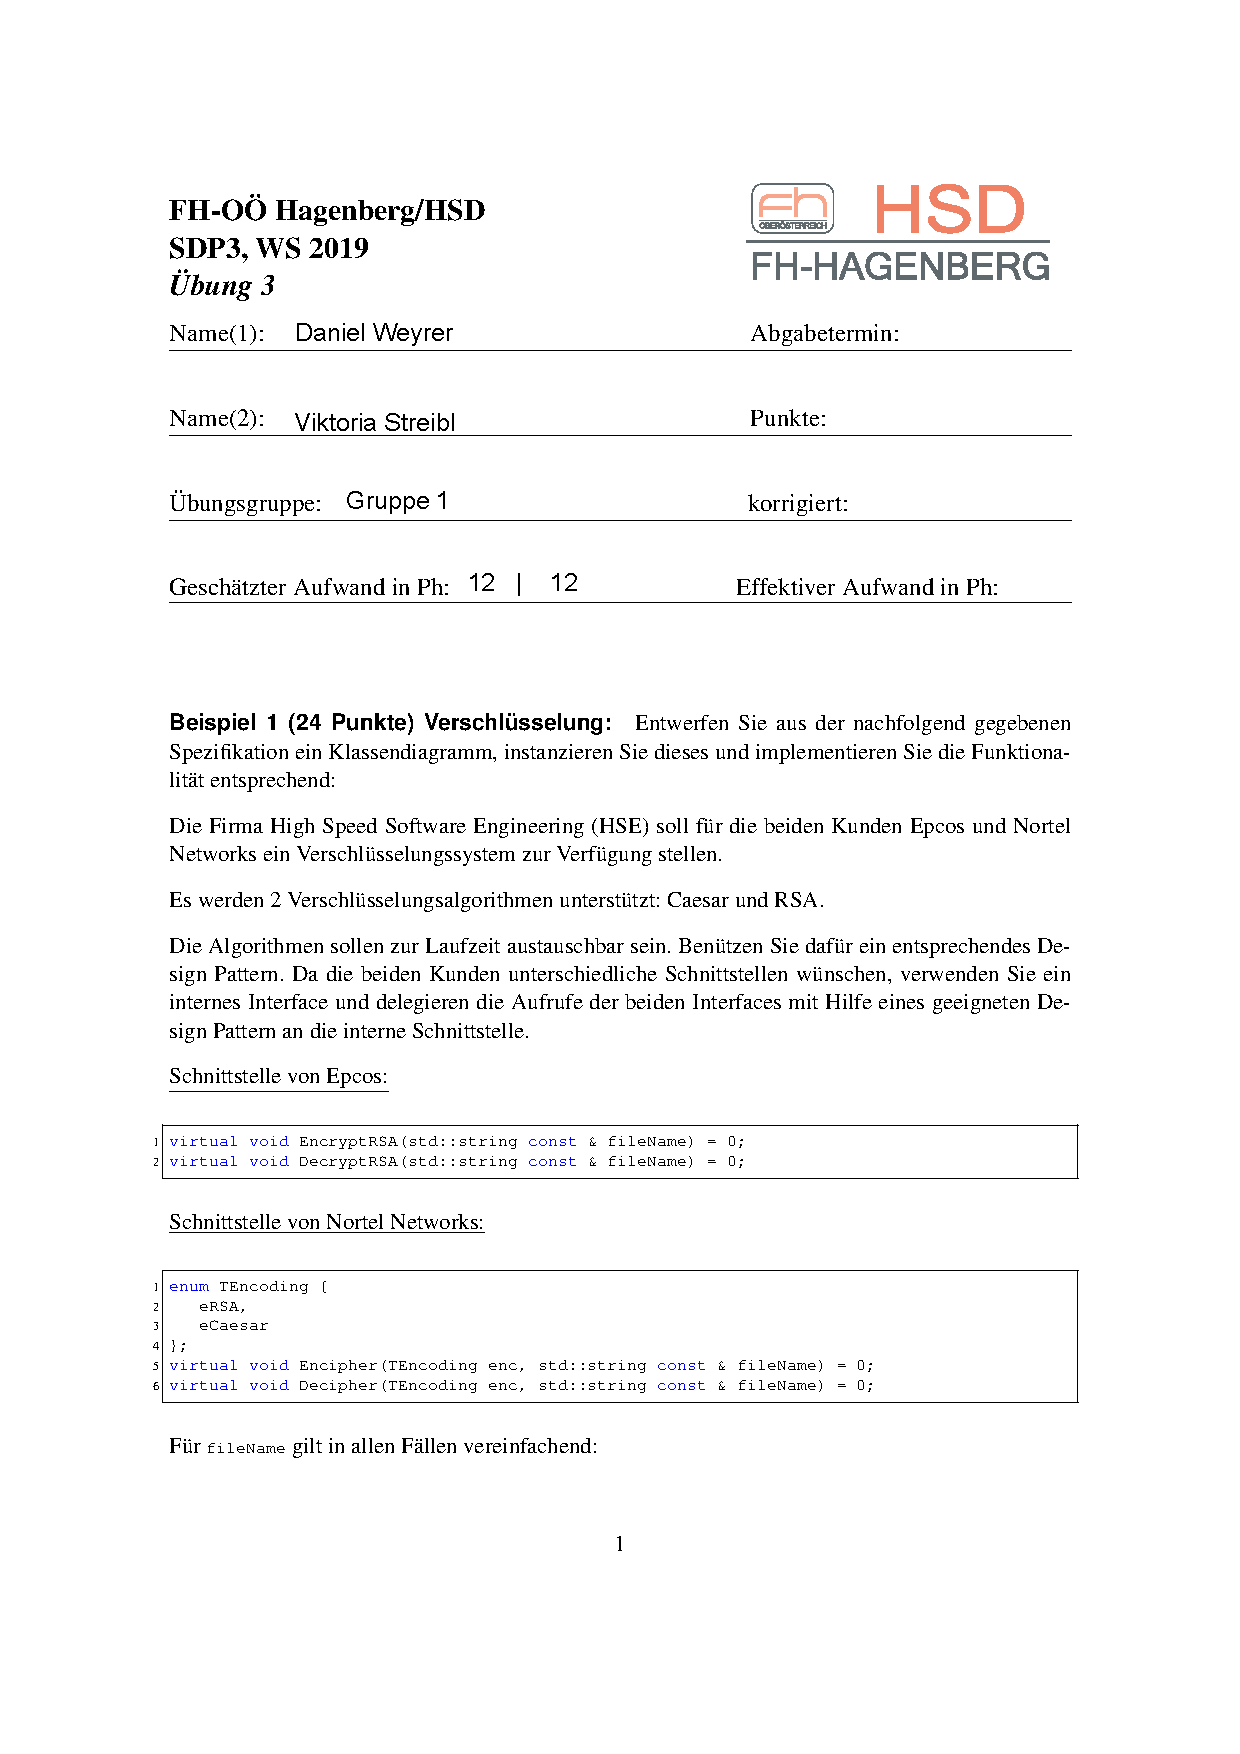
\includepdf[pages=-]{Angabe.pdf}

\title{SDP - Exercise 02} % Übungsname und Nummer angeben
\subtitle{winter semester 2019/20} % Semester angeben oder auskommentieren, falls nicht erwünscht
\author{
Viktoria Streibl - S1810306013\\
  Daniel Weyrer - S1820306044
} % Autorenname
\date{\today} % Das heutige Datum automatisch einfügen

\maketitle % Titelseite erstellen

\newpage
\tableofcontents % Inhaltsverzeichnis erstellen
\newpage

\ihead{Viktoria Streibl}
\ohead{Daniel Weyrer}
\chead{SDP3-UE Uebung 02}

\section{Organizational}
\subsection{Team}
\begin{itemize}
	\item Viktoria 	Streibl 		- 	S1810306013
	\item Daniel 	Weyrer		-	S1820306044
\end{itemize}

\subsection{Roles and responsibilities}
\subsubsection{Jointly}
\begin{itemize}
	\item Planning
	\item Documentation
	\item Systemdocumentation
	\item Class Diagram
\end{itemize}

\subsubsection{Viktoria Streibl}
\begin{itemize}
	\item Clients
	\subitem Client Nortel Networks
	\subitem Client Epos

	\item Interfaces
	\subitem IEpos
	\subitem INortelNetworks

	\item Adaptors
	\subitem AEpos
	\subitem ANorteNetworks
		
	\item Testdriver
	
\end{itemize}

\subsubsection{Daniel Weyrer}
\begin{itemize}
	\item Base Class Encryptor
	\item Derived Classes
		\subitem Class RSA
		\subitem Class Caesar
\end{itemize}

\subsection{Effort}

\subsubsection {Viktoria Streibl}
\begin{itemize}
	\item estimated: 12 ph 
	\item actually: XX ph
\end{itemize}

\subsubsection {Daniel Weyrer}
\begin{itemize}
	\item estimated: 12 ph 
	\item actually: 8 ph
\end{itemize}

\section{Requirenment Definition(System Specification)}
The two Companies Epos and Nortel Networks should get access to a new encryption tool via two independent interfaces (which are already given in the information sheet). As the algorithms should be changeable while running the program, we came up with the idea of two adaptors and one base class.

\section{System Design}
\subsection{Classdiagram}
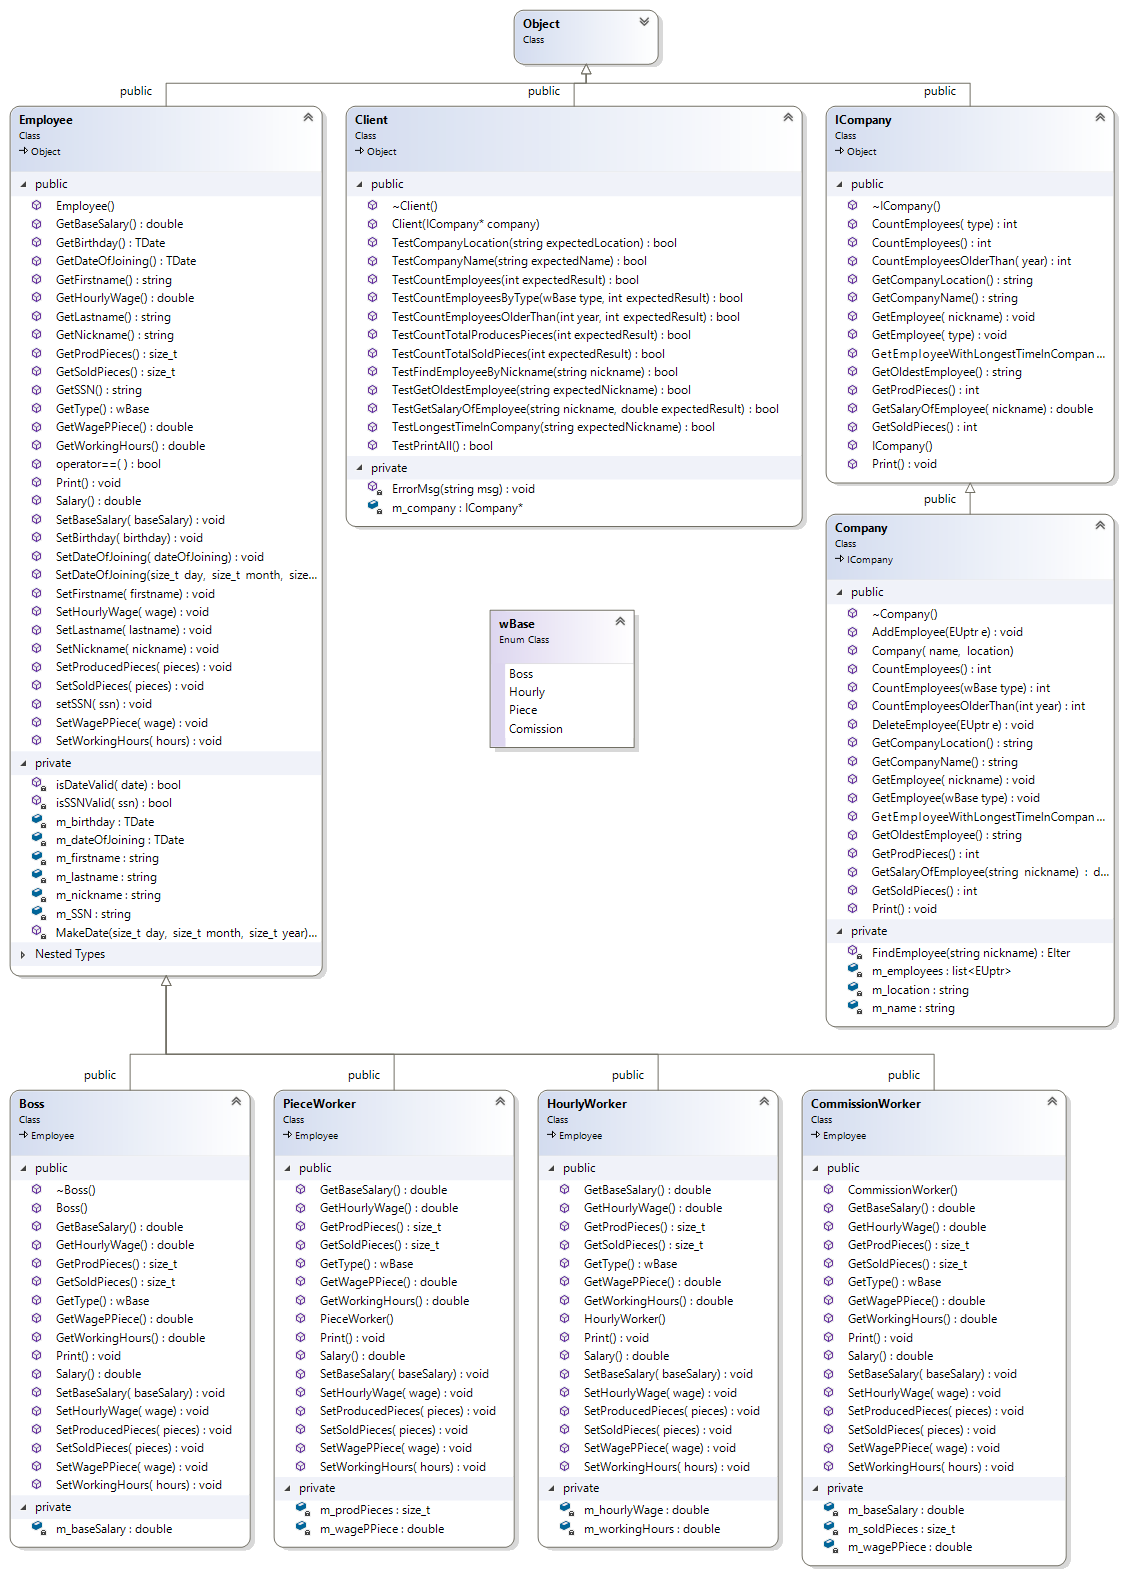
\includegraphics[scale=0.6, angle=90]{ClassDiagram}

\subsection{Design Decisions}
\subsubsection{Reading File into String}
The encryption is limited to 7-Bit ASCII-Values, which limits the encryption to plain text files. txt-files in the Megabyte-range are rare and the encryption method is not designed to deal with such many characters (+ it`s not safe, as we use a small key (RSA) and encrypt character by character).
\subsubsection{ASCII-Characters over 127}
\begin{itemize}
	\item Caesar-Encryption:	Characters with an ASCII-value over 127 cannot be encrypted due to the modulo division by 127, the Caesar-algorithm uses.	
	
	\subitem Encrypting: Characters are written unencrypted into the .Caesar with a warning written 
	\subitem in the command-line. 
	
	\subitem Decrypting: ASCII-values over 127 in a decrypted file (.caesar) are getting copied over to the decrypted.txt without any decryption. A warning is being delivered to the command-line
	
	\item RSA-Encryption
		\subitem Encrypting: Characters are being ignored and a warning is being delivered to the cmd, because we 				found no solution to handle values over 127 when decrypting a message. 
		
		\subitem Decrypting: All values are getting decrypted. If a decrypted-value is over 127 a warning is 							being delivered to the command-line and the decrypted-value is stored in the decrypted.txt
\end{itemize}

\subsubsection{Exception-Handling}
\begin{itemize}
	\item badalloc (thrown by e.g. string::reserve())
	\item std::exception (thrown by systemfunctions and user)
	\item unhandled exceptions
\end{itemize}

All Exceptions are thrown in the base-class (protected, non-public functions) and captured in the derived classes!
	
\section{Component Design}
\subsection{Class Client}
The Client simulate a person which use the interface.
The following functions tests the functionality:
\begin{itemize}
	\item Tests the company name
	\item Tests the company location
	\item Tests if it is possible to find a employee by nickname
	\item Tests if the employee which is search by his nickname is correct
	\item Counts all employees and check if it is correct
	\item Counts all employees of one type and check it
	\item Counts all produced pieces and check them
	\item Counts all sold pieces and check them
	\item Count how many employees are older than a specific year and check it
	\item Tests if the salary of an employee is correct
	\item Tests if the oldest employee is correct
	\item Check for the employee with is the oldest member
	\item Print all data of company and employees
\end{itemize}

All these methods are only for testing the functionality of Company. Furthermore, the Client gets the company with the constructor as ICompany.

\subsection{Client Epos}
\subsection{Client Nortel Networks}
\subsection{Interface IEpos}
\subsection{Interface INortelNetworks}
\subsection{Adaptor AEpos}
\subsection{ANortelNetworks}

\subsection{Class Encryptor}
Base Class, contains base-functionality such as:
\begin{itemize}
\item void GenFile(fileName, content)
\subitem Creates new File with the given Filename and writes the content into the file

\item string ReadFile(fileName)
\subitem Reads of the file with the given File-name into a string and returns the string.

\item string NewFileEnding(oldFileName, oldFileEnding, newFileEnding (, appendix)
\subitem Checks for correct file-ending of the file and creates a new one with the new file-extension and optional with an appendix (to create "filename decrypted.txt"). Throws an exception if the file has the wrong file-extension, returns string with new Filename (and extension) otherwise.

\end{itemize}
\subsection{Class Caesar}
\subsection{Class RSA}

\subsection{TestDriver}
The Testdriver test alle functions of the Client. It adds commisson worker, hourly worker, pieces worker and a boss.
The functions "TestLinzAG", "TestSequality" and "TestTractive" call the testing functions of client and check if everything worked.
The test-functions in Client returns a bool. If the bool returns false something didn't pass and this Testcase cannot get valid again.
It ouputs a error message if there was no successful run.

\newpage
\section{Test Protocol}


\subsection{Console Output}


\section{Source Code}

\subsection{ClientEpos}
\subsubsection{ClientEpos.h}
\sourceCode{./Encoding/Encoding/Client_Epos.h}
\subsubsection{ClientEpos.cpp}
\sourceCode{./Encoding/Encoding/Client_Epos.cpp}
\newpage
\subsection{Client Nortel Networks}
\subsubsection{ClientNortelNetworks.h}
\sourceCode{./Encoding/Encoding/Client_NortelNetworks.h}
\subsubsection{ClientNortelNetworks.h}
\sourceCode{./Encoding/Encoding/Client_NortelNetworks.cpp}
\newpage
\subsection{Interface IEpos}
\subsubsection{IEpos.h}
\sourceCode{./Encoding/Encoding/IEpos.h}

\subsection{Interface INortelNetworks}
\subsubsection{INortelNetworks.h}
\sourceCode{./Encoding/Encoding/INortelNetworks.h}
\newpage

\subsection{Adaptor AEpos}
\subsubsection{AEpos.h}
\sourceCode{./Encoding/Encoding/AEpos.h}
\subsubsection{AEpos.cpp}
\sourceCode{./Encoding/Encoding/AEpos.cpp}
\newpage
\subsection{ANortelNetworks}
\subsubsection{ANortelNetworks.h}
\sourceCode{./Encoding/Encoding/ANortelNetworks.h}
\subsubsection{ANortelNetworks.cpp}
\sourceCode{./Encoding/Encoding/ANortelNetworks.cpp}
\newpage

\subsection{Class Encryptor}
\subsubsection{Encryptor.h}
\sourceCode{./Encoding/Encoding/Encryptor.h}
\subsubsection{Encryptor.cpp}
\sourceCode{./Encoding/Encoding/Encryptor.cpp}
\newpage

\subsection{Class Caesar}
\subsubsection{Caesar.h}
\sourceCode{./Encoding/Encoding/Caesar.h}
\subsubsection{Caesar.cpp}
\sourceCode{./Encoding/Encoding/Caesar.cpp}
\newpage
\subsection{Class RSA}
\subsubsection{RSA.h}
\sourceCode{./Encoding/Encoding/RSA.h}
\subsubsection{RSA.cpp}
\sourceCode{./Encoding/Encoding/RSA.cpp}
\newpage

\subsection{TestDriver}
\subsubsection{TestDriver.h}
\sourceCode{./Encoding/Encoding/TestDriver.h}
\subsubsection{TestDriver.cpp}
\sourceCode{./Encoding/Encoding/TestDriver.cpp}
\newpage
% Um Quellcode einzufügen einfach diesen Befehl verwenden:
%\sourceCode{Relativer/Pfad/zum/SourceCode.Endung}

\end{document}